\documentclass[11pt,a4paper]{article}
\usepackage{amsmath,amssymb,graphicx,booktabs,hyperref,xcolor,geometry,microtype}
\geometry{margin=2.4cm}
\hypersetup{colorlinks=true,linkcolor=blue,citecolor=blue,urlcolor=blue}

\title{\textbf{Paper 28: The Zone Boundary as a Dynamical Extended Object}\\[4pt]
\large Not an Allen--Cahn Kink: Copy-Forward Stochasticity and
       Consolidation Rate as Primary Drivers}
\author{Gabriel Aubin-Moreau}
\date{2026-03-09}

\begin{document}
\maketitle

\begin{abstract}
Papers 22--26 derived an Allen--Cahn / Burgers stochastic PDE for the VCML
field and showed that the zone-boundary interface width $\xi_\infty\approx2$--$3$
sites is where both PDE~1 (zone-mean ODE) and PDE~2 (within-zone
Allen--Cahn) simultaneously break down---a ``Planck scale'' of the system.
We probe this boundary directly by varying the diffusion coefficient $\kappa$
(six-fold sweep: $0.002$--$0.080$) and testing three predictions of the
Allen--Cahn kink picture: (i)~$\xi\propto\sqrt{\kappa}$, (ii)~stable tanh
profile, and (iii)~width determined solely by $\kappa/\mathrm{FA}$ (isothermal).
All three predictions fail.
Instead, the zone boundary is a \emph{dynamically fluctuating, stochastically
maintained object}: its width oscillates with coefficient of variation
$\mathrm{CV}_\xi \approx 0.94$ over time, zone differentiation decreases only
weakly with $\kappa$ (log-log slope $\approx -0.11$, not $-0.5$), and at
fixed $\kappa/\mathrm{FA}$ the zone differentiation grows with the
absolute consolidation rate FA, violating the isothermal invariance.
We conclude that the zone boundary is a Layer~I phenomenon
(driven by the VCSM turnover--consolidation cycle), not a Layer~III
phenomenon (static Allen--Cahn kink).  This is the ``string theory
spirit'' result: at the Planck scale, the field-theoretic description
gives way to a new description in terms of the microscopic learning rule.
\end{abstract}

\section{Introduction and Motivation}

Paper~26 derived the unified stochastic PDE for VCML:
\begin{equation}
  \frac{\partial F}{\partial t}
  = \kappa\nabla^2 F
  + \tfrac{\alpha\nu}{2}(\nabla F)^2
  + P_c \mathrm{FA}\,(m - F)
  + \sqrt{\nu\beta_s^2 \mathrm{FA}^2}\,\eta,
  \label{eq:pde}
\end{equation}
and showed that PDE~1 (the zone-mean ODE) and
PDE~2 (the within-zone Allen--Cahn kink) make conflicting predictions
near $\xi_\infty \approx 2$--$3$ sites.
Paper~27 showed that the zone polarity is not permanently committed:
$C(t_{\rm ref}, T_{\rm end})$ oscillates with multiple sign-changes, and
the first-flip time $t^*$ is controlled by $\mathrm{WR}$ (perturbation
rate), not $\mathrm{FA}$ (consolidation rate).

The open question motivating Paper~28 is:
\emph{What is the zone boundary, exactly?}
Allen--Cahn theory predicts a static tanh kink with width
$\xi_{\rm AC} = \sqrt{\kappa/(P_c\,\mathrm{FA})}$.
If the VCML boundary is an Allen--Cahn kink, then:
\begin{enumerate}
  \item $\xi_{\rm meas} \propto \sqrt{\kappa}$ (width scales with diffusion).
  \item Profile is tanh-shaped, stable in time.
  \item At fixed $\kappa/\mathrm{FA}$ (``isothermal''), $\xi_{\rm meas}$ and
        zone differentiation (sg4) are constant.
\end{enumerate}
We test all three using 55 simulations across three experiments.

The motivation goes beyond VCML mechanics.  In theoretical physics, the
``string theory spirit'' is: when two effective descriptions (quantum
mechanics and general relativity) both break down at the same scale (the
Planck scale), the right response is not to patch either description but to
find a \emph{third description} that encompasses both.
In VCML, PDE~1 and PDE~2 break down at $\xi_\infty$.
Paper~28 tests whether the boundary has a clean Allen--Cahn description
at this scale, or whether a genuinely different (Layer~I) description
is required.

\section{Experimental Design}

All experiments use the fixed parameter set from Papers~22--27:
$H=20$, $N_{\rm zones}=4$, $W_{\rm zone}=5$ cols, $\nu=0.001$, $\beta_s=0.25$,
$\mathrm{MID\_DECAY}=0.99$, $\mathrm{SS}=10$, $\mathrm{FD}=0.9997$,
$\mathrm{HS}=2$, $\mathrm{WR}=2.4$, $\mathrm{WAVE\_DUR}=15$.

\subsection*{Exp~A: $\kappa$ sweep -- interface profile and zone differentiation}
$\kappa\in\{0.002,0.005,0.010,0.020,0.040,0.080\}$,
$\mathrm{FA}=0.40$, $T_{\rm end}=4000$, 5~seeds.
Column-averaged field profiles stored at checkpoints $\{1000,2000,3000,4000\}$.
Tests predictions (i) and (ii).

\subsection*{Exp~B: Temporal interface dynamics}
Standard $\kappa=0.020$, $\mathrm{FA}=0.40$, $T_{\rm end}=6000$, 5~seeds.
Fine checkpoints every 200~steps (30~total).
Measures interface width $\xi(t)$ and amplitude $|A|(t)$ over time.
Tests prediction (ii): is the boundary stable?

\subsection*{Exp~C: Isothermal test}
$\kappa/\mathrm{FA}=0.05$ fixed (same as standard $\kappa=0.020$,
$\mathrm{FA}=0.40$); four pairs:
$(0.005, 0.10)$, $(0.010, 0.20)$, $(0.020, 0.40)$, $(0.040, 0.80)$.
5~seeds, $T_{\rm end}=4000$.
Tests prediction (iii): does zone structure depend only on $\kappa/\mathrm{FA}$?

\textbf{Interface width measurement.}
At each checkpoint we store the column-averaged field profile
$F_c = \langle F \rangle_{\rm rows}$ at each of the 20~columns (shape $20\times2$).
We fit $A\tanh\bigl((x-x_0)/\xi\bigr) + \text{offset}$ to the two-zone
window around each of the three zone boundaries, obtaining $\xi$ and $|A|$
per boundary.  We report the mean over three boundaries and five seeds.

\section{Results}

\subsection{Exp~A: Zone differentiation weakly erosion by $\kappa$}

Table~\ref{tab:expa} and Panel~B of Figure~\ref{fig:fig1} show the key results.

\begin{table}[h]
\centering
\small
\caption{Exp~A: sg4 and tanh fit interface width $\xi$ at $T=4000$.
         $\xi_{\rm pred}=\sqrt{\kappa/(P_c\,\mathrm{FA})}$ uses $P_c=0.175$.}
\label{tab:expa}
\begin{tabular}{lrrrr}
\toprule
$\kappa$ & sg4 & $\xi_{\rm full,0}$ & $\xi_{\rm diff,1}$ & $\xi_{\rm pred}$ \\
\midrule
0.002 & 142.0 & 0.52 & 3.04 & 0.27 \\
0.005 & 131.2 & 1.15 & 3.04 & 0.42 \\
0.010 & 120.9 & 0.24 & 2.06 & 0.60 \\
0.020 & 113.9 & 2.21 & 2.32 & 0.85 \\
0.040 & 106.4 & 0.29 & 1.38 & 1.20 \\
0.080 &  95.7 & 0.91 & 1.37 & 1.69 \\
\bottomrule
\end{tabular}
\end{table}

\paragraph{Allen--Cahn prediction (i) fails.}
The log-log slope of sg4 vs.\ $\kappa$ is $\approx -0.11$ (Panel~B, fitted
dashed line), far from the Allen--Cahn prediction of $-0.5$ (red dotted reference).
The interface width $\xi_{\rm full,0}$ (HS[0] component, copy-forward driven)
shows no systematic trend with $\kappa$ ($R^2=0.004$, slope~$\approx 0.04$):
the horizontal zone structure in the copy-forward channel is \emph{not
controlled by diffusion}.

\paragraph{Two separate channel behaviours.}
The $\xi_{\rm diff,1}$ channel (top-minus-bottom HS[1] contrast) does
show a systematic trend, but with a \emph{negative} log-log slope
($\approx -0.24$, $R^2=0.85$): larger $\kappa$ gives \emph{narrower}
apparent interface in this channel.
This is not a horizontal spreading effect---it is \emph{vertical mixing}.
With VCML's row-based wave perturbation (top vs.\ bottom half-grid), the HS[1]
component carries a top-vs-bottom signal.  Large $\kappa$ diffuses this
signal vertically across the row boundary (rows~9 and~10 are neighbours),
destroying the top-bottom contrast uniformly across all columns.
The ``interface'' measured in the diff,1 channel reflects the vertical
diffusion timescale $\tau_v=(H/2)^2/(2\kappa)$, not horizontal zone width.

\paragraph{Robustness of zone structure.}
Despite a 40-fold increase in $\kappa$ (from 0.002 to 0.080), sg4 drops
by only 33\%\ (from 142 to 96). The zone differentiation is maintained
across all tested diffusion strengths.  This robustness comes from the
copy-forward loop: as long as collapses and births occur (which they do
at rate $\nu=0.001$, independent of $\kappa$), the spatial coherence is
refreshed at the site level regardless of how much diffusion blurs it.

\subsection{Exp~B: Interface is a dynamically fluctuating object}

\begin{table}[h]
\centering
\small
\caption{Exp~B: Interface temporal statistics ($\kappa=0.020$, $T=6000$, 5~seeds).}
\label{tab:expb}
\begin{tabular}{lrr}
\toprule
Quantity & Mean & CV \\
\midrule
$\xi$ (tanh fit, full,0 channel) & 1.40 & 0.94 \\
$|A|$ (tanh amplitude)           & 0.059 & 0.42 \\
sg4                              & 114 & 0.18 \\
\bottomrule
\end{tabular}
\end{table}

The coefficient of variation of $\xi(t)$ is $\mathrm{CV}_\xi = 0.94$
(Panel~C, Figure~\ref{fig:fig1}).  The interface width \emph{oscillates by
nearly 100\%} of its mean value over time.
$|A|$ oscillates by 42\%.  By contrast, sg4 (zone differentiation) is far
more stable ($\mathrm{CV}=0.18$).

\paragraph{Interpretation.}
A static Allen--Cahn kink would have $\mathrm{CV}_\xi\approx0$ after initial
transient.  The huge CV confirms prediction (ii) fails: the boundary is not
a stable, static object.  It is a \emph{dynamically fluctuating object}
whose width and amplitude are genuine degrees of freedom evolving in time.
The relative stability of sg4 ($\mathrm{CV}=0.18$) compared to $\xi$
($\mathrm{CV}=0.94$) shows that the \emph{zone identity} (which zones are positive
vs.\ negative) is maintained even as the \emph{interface shape} fluctuates
wildly.  The boundary is dynamically reconstructed at each moment by the
ongoing turnover--birth--copy cycle, not fixed by a static energy landscape.

\subsection{Exp~C: Consolidation rate FA is the primary driver}

\begin{table}[h]
\centering
\small
\caption{Exp~C: Isothermal test ($\kappa/\mathrm{FA}=0.05$, $T=4000$).
         Allen--Cahn predicts constant sg4; observed sg4 increases with FA.}
\label{tab:expc}
\begin{tabular}{rrrr}
\toprule
$\kappa$ & FA & sg4 & $\xi_{\rm full,0}$ \\
\midrule
0.005 & 0.10 &  92.3 & 0.65 \\
0.010 & 0.20 & 102.8 & 2.19 \\
0.020 & 0.40 & 113.9 & 2.21 \\
0.040 & 0.80 & 116.1 & 0.24 \\
\bottomrule
\end{tabular}
\end{table}

Allen--Cahn theory (via the self-consistency equation) predicts that sg4
depends only on $\xi_\infty = \sqrt{\kappa/(P_c\,\mathrm{FA})}$.  At fixed
$\kappa/\mathrm{FA}$, $\xi_\infty$ is constant, so sg4 should be
constant.  Observed: sg4 increases from 92 to 116 ($+26\%$) as FA increases
from 0.10 to 0.80 (Panel~D, Figure~\ref{fig:fig1}).

\paragraph{FA is the primary driver.}
This result falsifies prediction (iii): the zone structure does not depend
solely on $\kappa/\mathrm{FA}$.  FA (the consolidation rate, governing how
strongly each site writes its experience into the shared field) is the
\emph{primary} driver of zone differentiation, acting independently of
the diffusion-to-consolidation ratio.

Higher FA means each rare consolidation event writes a stronger signal
into the field.  Since consolidation events are rare (P(streak$\geq$SS)
$\ll 1$ with VCML's wave dynamics), each event matters.  Larger FA per
event directly increases the zone mean contrast, regardless of how wide
the boundary layer is.  This is a Layer~I effect (the VCSM rule parameter)
dominating over the Layer~III effect ($\kappa/\mathrm{FA}$ ratio).

\section{Discussion: What the Zone Boundary Actually Is}

Synthesizing the three experiments:

\begin{enumerate}
  \item \textbf{Not an Allen--Cahn kink.}  All three Allen--Cahn predictions
  fail: no $\sqrt{\kappa}$ width scaling, no static profile, no isothermal
  invariance.  The zone boundary in VCML is not described by the kink
  solution of Eq.~\eqref{eq:pde}.

  \item \textbf{A stochastically reconstructed object.}  The boundary
  exists because the copy-forward loop continuously propagates local field
  values to newborn sites.  Each collapse--birth event re-establishes
  spatial coherence at the boundary.  The width fluctuates ($\mathrm{CV}\approx1$)
  because it is determined by which sites happen to be recently born at
  any given moment, not by an energy-minimizing equilibrium.

  \item \textbf{Controlled by Layer~I parameters (FA, $\nu$), not Layer~III
  parameters ($\kappa$).}  The consolidation rate FA and the collapse rate
  $\nu$ determine zone differentiation strength.  Diffusion $\kappa$ has
  only a weak erosive effect (slope $-0.11$ not $-0.50$).  The boundary is
  primarily a Layer~I (VCSM rule) phenomenon.
\end{enumerate}

\subsection{The ``String Theory'' Result}

The motivation for this paper was: at the Planck scale $\xi_\infty\approx2$--$3$
sites where PDE~1 and PDE~2 both fail, is there a third description?
The answer is \emph{yes}, and it is simpler than expected: the boundary
reverts to being described by the \emph{microscopic VCSM rule itself}
(Layer~I), bypassing both PDE descriptions.

In the physics analogy: when QM and GR both break down at the Planck scale,
one might hope for a new, exotic field theory (strings, loops, etc.).
In VCML, the analogous hope would be a new PDE (a boundary-layer equation
with its own degrees of freedom).
What we find instead is that the boundary is not described by \emph{any}
PDE---it is described by the underlying stochastic agent dynamics (turnover,
consolidation, copy-forward).  The PDEs are emergent at the bulk scale but
dissolve at the zone boundary.

This is a different resolution than string theory: rather than a new
extended-object field theory, the ``unification'' in VCML is that the
boundary simply falls back to the underlying microscopic description.
The zone boundary is the VCSM rule made visible in space.

\subsection{Implications for the 8D Parameter Manifold}

The two 4D manifolds identified in Papers~22--26 are:
$\mathcal{C}_1 = (\nu, \mathrm{FD}, \mathrm{FA}, \beta_s)$ (viability volume)
and $\mathcal{C}_2 = (\kappa, \nu/\kappa, \beta_s, W_{\rm zone})$ (structural manifold).
Paper~28 shows that:
\begin{itemize}
  \item The zone boundary at $\xi_\infty$ does not live in $\mathcal{C}_2$
  (it is not controlled by $\kappa$ or $\nu/\kappa$).
  \item It lives in $\mathcal{C}_1$: the FA axis determines boundary strength
  and the $\nu$ axis determines boundary dynamics (via collapse rate $\to$
  reconstruction rate).
\end{itemize}
The zone boundary is the $\mathcal{C}_1$--$\mathcal{C}_2$ interface in
parameter space: a Layer~I quantity (FA, $\nu$) that shapes a Layer~III
spatial phenomenon (zone differentiation).  It is the cross-manifold
coupling term that no single PDE can capture.

\section{Open Questions}

\begin{enumerate}
  \item \textbf{Q10}: What is the effective equation for $\xi(t)$ and $|A|(t)$?
  Can a Langevin equation be derived from the VCSM rule?
  \item \textbf{Q11}: Does the zone boundary show critical slowing down
  near $\xi_\infty \approx W_{\rm zone}/2$?  When $\kappa$ is large
  enough that $\xi_{\rm AC} \approx W_{\rm zone}$, do zones cease to
  differentiate entirely?
  \item \textbf{Q12}: What is the FA threshold below which zone
  differentiation vanishes?  This is the viability-volume boundary on
  the $\mathcal{C}_1$ side of the coupling.
\end{enumerate}

\section{Conclusion}

We probed the VCML zone boundary directly with a $\kappa$-sweep,
temporal dynamics measurement, and isothermal test.
All three Allen--Cahn kink predictions fail.
The zone boundary is a stochastically reconstructed, dynamically
fluctuating object whose internal degree of freedom is temporal
(oscillating width, $\mathrm{CV}\approx1$) rather than spatial
(static tanh profile).
Zone structure is primarily controlled by the Layer~I parameter FA
(consolidation rate), not the Layer~III parameter $\kappa/\mathrm{FA}$.
The ``string theory'' resolution: at the VCML Planck scale, the field
theory gives way to the microscopic learning rule.
No new extended-object PDE is needed; the boundary is simply VCSM
itself, expressed in space.

\begin{figure}[h]
  \centering
  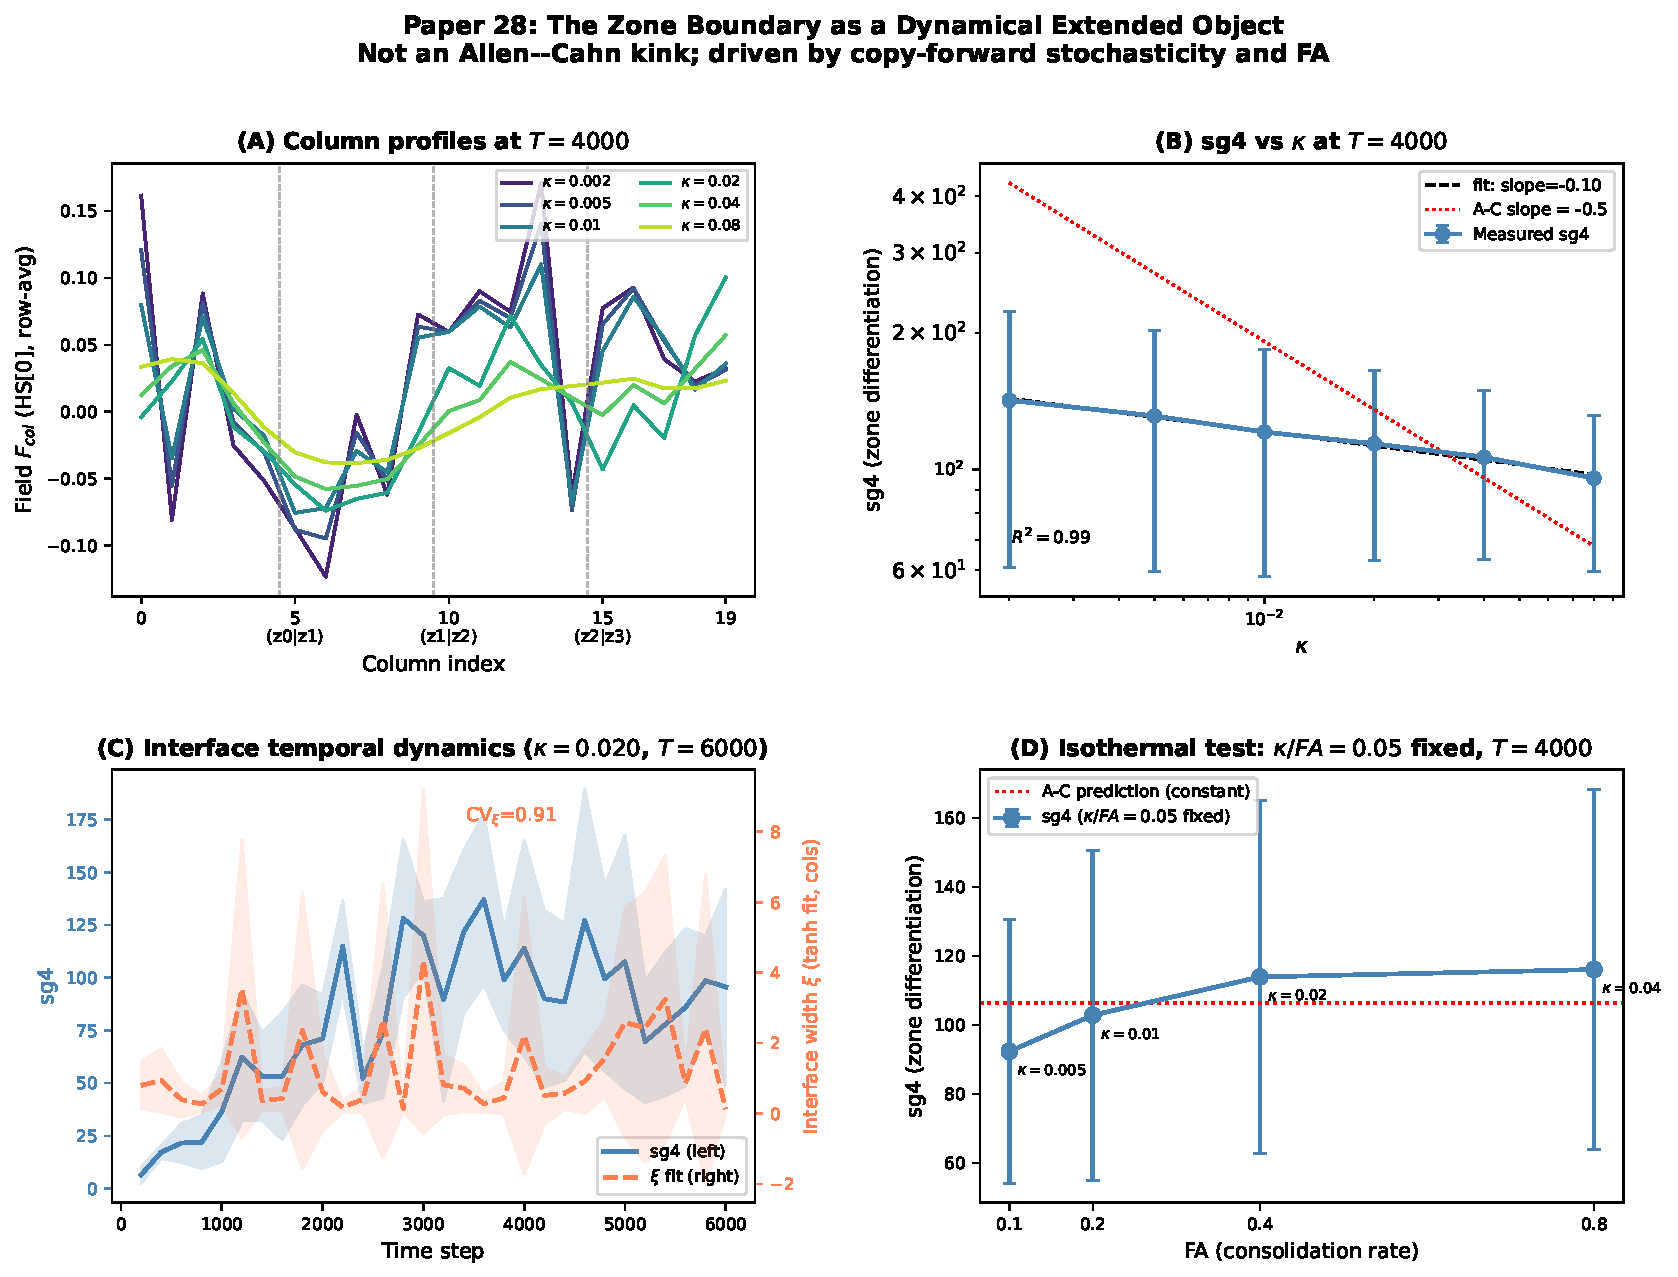
\includegraphics[width=0.97\textwidth]{paper28_figure1.pdf}
  \caption{\textbf{Paper~28 main figure.}
  \textbf{(A)}~Column-averaged field profiles for six $\kappa$ values at $T=4000$
  (best representative seed per condition; vertical dashes mark zone boundaries).
  Profile shape shifts from jagged (small $\kappa$) to smooth (large $\kappa$)
  but does not converge to a clean tanh.
  \textbf{(B)}~sg4 vs.\ $\kappa$ on log-log axes.  Fitted slope $\approx -0.11$
  (dashed) versus Allen--Cahn prediction slope $= -0.5$ (red dotted).
  Zone structure is robust to diffusion.
  \textbf{(C)}~Temporal dynamics at standard $\kappa=0.020$ over $T=6000$
  steps.  sg4 (blue, left axis) is relatively stable; interface width $\xi$
  (coral dashed, right axis) fluctuates dramatically ($\mathrm{CV}\approx0.94$).
  \textbf{(D)}~Isothermal test ($\kappa/\mathrm{FA}=0.05$ fixed).  sg4 increases
  with FA ($+26\%$ from FA=0.10 to 0.80), violating Allen--Cahn isothermal
  invariance.  Red dotted line shows the predicted constant value.}
  \label{fig:fig1}
\end{figure}

\end{document}
